%% Type de document et encodage de la police
\documentclass[a4paper]{article}
\usepackage[utf8x]{inputenc}

%% Initialise la taille des pages et des marges
\usepackage[a4paper,top=3cm,bottom=3cm,left=2cm,right=2cm,marginparwidth=1.75cm]{geometry}

%% Packs utiles
\usepackage{amsmath}
\usepackage{graphicx}
\usepackage[colorinlistoftodos]{todonotes}
\usepackage[colorlinks=true, allcolors=black]{hyperref}
\usepackage{fourier-orns}
\usepackage{titlesec}
\usepackage{fancyhdr}
\usepackage{fancyvrb}
\usepackage{array}


%% Packs utiles pour la manipulation d'image
\usepackage{wallpaper}
\usepackage{amsfonts}
\usepackage{amssymb}
\usepackage{eso-pic}
\usepackage{multicol}

%% \setlength
\setlength{\parindent}{0.5cm}

%% \thefootnote
\renewcommand{\thefootnote}{\*}
\pagestyle{fancy} 
\setcounter{tocdepth}{5}
\renewcommand{\thefootnote}{\arabic{footnote}}

%% \headrulewidth
\renewcommand{\headrulewidth}{1pt}
\fancyhead[C]{} 
\fancyhead[L]{}
\fancyhead[R]{\footnotesize{\leftmark}}

%% \footrulewidth
\renewcommand{\footrulewidth}{1pt}
\fancyfoot[C]{} 
\fancyhead[L]{}
\fancyfoot[R]{\thepage}

%% definecolor
\definecolor{Zgris}{rgb}{0.87,0.85,0.85}

%% Pour mettre des lignes à gauche et à droite d'un exemple
\usepackage{mdframed}
\newmdenv[
    topline=false,
    bottomline=false,
    skipabove=\topsep,
    skipbelow=\topsep
]{siderules}

\renewcommand{\arraystretch}{1.2} %% row 20% longer

%% Redéfinition de la colonne d'un tableau pour que ses éléments soient centrés sur l'axe vertical
%% Implique l'utilisation de \tabularnewline à la place de \\ pour terminer une ligne du tableau
\newcolumntype{M}[1]{>{\raggedright}m{#1}}

%% Pack Tikz pour les diagrammes
\usepackage{tikz}
\usetikzlibrary{shapes.geometric, arrows, shapes, shapes.multipart, decorations.pathmorphing, backgrounds, positioning, fit, petri}


%% Définition des noeuds (flowchart)
\tikzstyle{start} = [rectangle, rounded corners, minimum width = 3cm, minimum
height = 1cm, text centered, fill = red!30]
\tikzstyle{input} = [trapezium, trapezium left angle = 70, trapezium right angle = 110,
minimum width = 3cm, minimum height = 1cm, text centered, text width = 3.5cm, fill = blue!30]
\tikzstyle{instruction} = [rectangle, minimum width = 3cm, minimum height = 1cm, text
centered, text width = 3cm, fill = orange!30]
\tikzstyle{condition} = [diamond, minimum width = 3cm, minimum height = 1cm, text
centered, draw = black, fill = green!30]
\tikzstyle{arrow} = [thick, ->, >=stealth]
\tikzset{
    function/.style = {
        draw,
        rectangle split,
        rectangle split horizontal,
        rectangle split parts=3,
        minimum height=1cm, text centered, draw=black, fill=yellow!30
    }
}



\title{Analyse II}
\author{Grégoire Roumache}
\date{Juillet 2017}

\begin{document}

\maketitle
























\section{Suites et séries}






\begin{center}
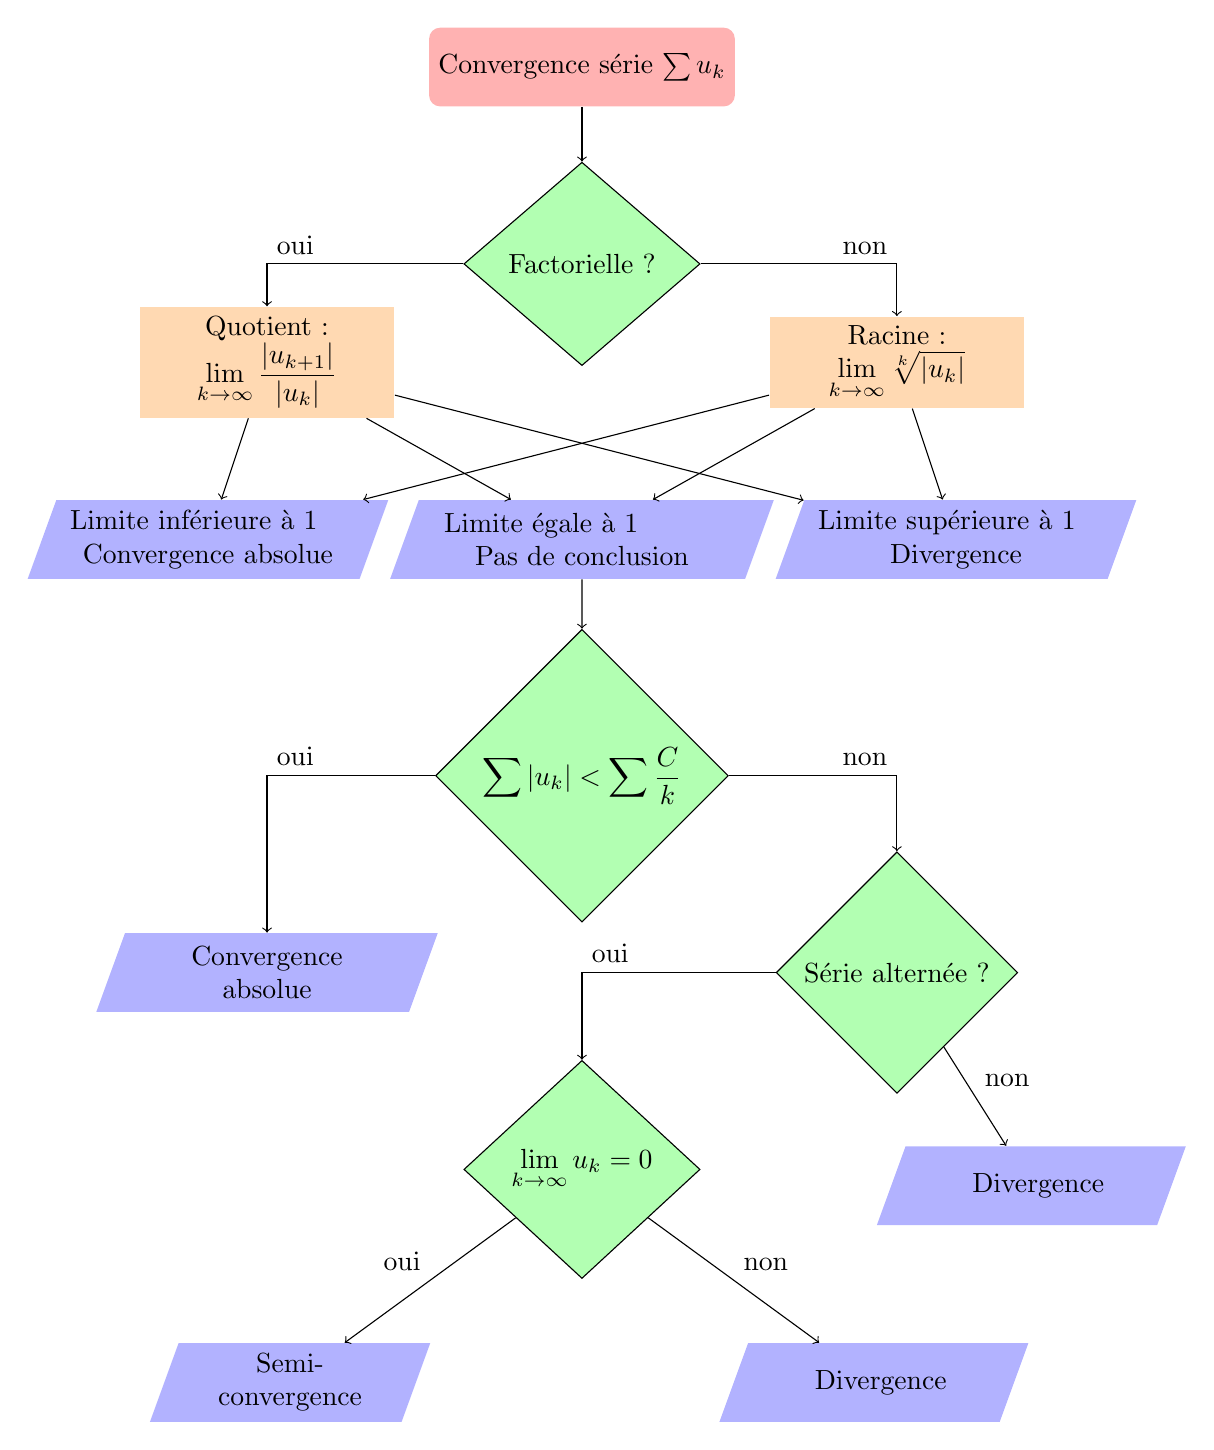
\begin{tikzpicture}

    \node (start) [start] at (0,0) {Convergence série $ \sum u_k $};
    \node (decision) [condition] at (0,-2.5) {Factorielle ?};
    \node (oui1) [instruction] at (-4,-3.75) {Quotient : \\ $\displaystyle \lim_{k \to \infty} \frac{|u_{k+1}|}{|u_k|} $};
    \node (non1) [instruction] at (+4,-3.75) {Racine : \\ $\displaystyle \lim_{k \to \infty} \sqrt[k]{|u_k|} $};

    \node (inferieur) [input] at (-4.75,-6) {Limite inférieure à 1 \newline Convergence absolue};
    \node (egal) [input] at (0,-6) {Limite égale à 1 \newline Pas de conclusion};
    \node (superieur) [input] at (4.75,-6) {Limite supérieure à 1 \newline Divergence};

    \node (decision2) [condition] at (0,-9) {$\displaystyle \sum |u_k| < \sum \frac{C}{k} $};
    \node (oui2) [input, text width=3cm] at (-4,-11.5) {Convergence absolue};
    \node (non2) [condition] at (4,-11.5) {Série alternée ?};

    \node (oui3) [condition, below of = decision, yshift = -10.5cm] {$\displaystyle \lim_{k \to \infty} u_k = 0 $};
    \node (non3) [input, below right of = non2, xshift = 1cm, yshift = -2cm, text width = 1.5cm] {Divergence};

    \node (oui4) [input, below left of = oui3, xshift = -3cm, yshift = -2cm, text width = 2.5cm] {Semi-convergence};
    \node (non4) [input, below right of = oui3, xshift = 3cm, yshift = -2cm, text width = 1.5cm] {Divergence};

    \draw[->] (start) -- (decision);
    \draw[->] (decision) -| node[anchor = south west]{oui} (oui1);
    \draw[->] (decision) -| node[anchor = south east]{non} (non1);
    \draw[->] (oui1) -- (superieur);
    \draw[->] (oui1) -- (egal);
    \draw[->] (oui1) -- (inferieur);
    \draw[->] (non1) -- (superieur);
    \draw[->] (non1) -- (egal);
    \draw[->] (non1) -- (inferieur);
    \draw[->] (egal) -- (decision2);
    \draw[->] (decision2) -| node[anchor = south west]{oui} (oui2);
    \draw[->] (decision2) -| node[anchor = south east]{non} (non2);
    \draw[->] (non2) -| node[anchor = south west]{oui} (oui3);
    \draw[->] (non2) -- node[anchor = south west]{non} (non3);
    \draw[->] (oui3) -- node[anchor = south east]{oui} (oui4);
    \draw[->] (oui3) -- node[anchor = south west]{non} (non4);

\end{tikzpicture}
\end{center}













\newpage



















\begin{itemize}






%% Série arithmétique
\item Une série arithmétique est de la forme : $\displaystyle S_n = \sum_{k=0}^{n-1} u_k = \sum_{k=0}^{n-1} (a + k d) = n \frac{1}{2} \Big( a + [a + (n - 1) d ] \Big) $. \\ On retient que l'on multiplie \emph{n} (le nombre de termes) à la valeur moyenne de $ u_k $ qui est la somme du premier terme ($ a $) et du dernier ($ a + (n - 1) d $) divisée par deux.





%% Série géométrique
\item Une série géométrique est de la forme : $\displaystyle S_n = \sum_{k=0}^{n-1} u_k = \sum_{k=0}^{n-1} a r^k = \sum_{k=0}^{n-1} \frac{a (1 - r^n)}{1 - r} $. \\ On peut visualiser ceci intuitivement en faisant le raisonnement : \[ (1 - r) (1 + r) = 1 - r^2 \]
\[ (1 - r) (1 + r + r^2) = 1 - r^3 \]
Et de manière générale : \quad $\displaystyle (1 - r) (1 + r + ... + r^{n-1}) = 1 - r^n $ \\
Lorsque $ n = \infty $ et que $ |r| < 1 $, la série devient : $\displaystyle S = \sum_{k=0}^{\infty} u_k = \sum_{k=0}^{\infty} a r^k = \frac{a}{1 - r} $





%% Critère de Cauchy pour la convergence des séries
\item Critère de Cauchy pour la convergence des séries : Une série $\displaystyle \sum_{k=1}^{\infty} u_k, \quad u_k \in \mathbb{C}, \; k \in \mathbb{N}_0 $ est convergente si et seulement si, 
\[ (\forall \epsilon > 0) (\exists N \in \mathbb{N}) (\forall q \geq p \geq N) : \Bigg| \sum_{k=p}^{q} u_k \Bigg| \leq \epsilon \]
C'est-à-dire, que l'on retient : 
\begin{itemize}
\item On décide que $ \epsilon $ peut prendre TOUTES les valeurs dans l'intervalle $ ]0, + \infty[ $ et le module de la série ($ u_p + u_{p+1} + ... + u_q $) doit y être inférieur. $ \epsilon $ peut notamment prendre une valeur infiniment petite (strictement supérieure à zéro).
\item Éventuellement, on peut trouver un nombre de termes \emph{N} tel que la somme de $ u_p $ ($ p \geq N $) à $ u_k $ ($ p \geq q $) est inférieure à $ \epsilon $. Dans le cas où \emph{p} et \emph{q} ont des valeurs "extrêmes", on a la somme :  $\displaystyle S = \sum_{k=p}^{q} u_k = \sum_{k=N}^{\infty} u_k $.
\end{itemize}

\begin{center}
\begin{tikzpicture}
    \draw[->] (0.25, 0) -- (8, 0) node[right] {$x$};
    \draw[->] (1.25, -1) -- (1.25, 4.2) node[above] {$y$};
    \draw[scale = 0.5, domain = 3:16, smooth, variable = \x, blue] plot ({\x}, {50/(\x*\x});
    \draw[-] (1.25, 2) node[left] {$\epsilon$} -- (8, 2);
    \draw[-] (4, 0) node[below] {$N$} -- (4, 1);
    \draw[-] (4, 1) node[below right, xshift = 1.5cm] {$ \Big| \sum u_k \Big| $} -- (8, 1);
\end{tikzpicture}
\end{center}






%% Critère de la racine de Cauchy
\item Critère de la racine de Cauchy : 
\[
\left.
    \begin{aligned}
        \lim_{k \to \infty} u_k^{1/k} > 1 \\
        \lim_{k \to \infty} u_k^{1/k} = 1^+
    \end{aligned}
\right\}
\qquad \sum_{k=1}^{\infty} u_k \text{ diverge }
\]





%% Critère du quotient de D'Alembert
\item Critère du quotient de D'Alembert : 
\[
\left.
    \begin{aligned}
        \lim_{k \to \infty} \frac{u_{k+1}}{u_k} > 1 \\
        \lim_{k \to \infty} \frac{u_{k+1}}{u_k} = 1^+
    \end{aligned}
\right\}
\qquad \sum_{k=1}^{\infty} u_k \text{ diverge }
\]





%% Remarque sur les critères de la racine et du quotient
\item Remarque sur les critères de la racine et du quotient : Ces deux critères ne permettent pas de donner une conclusion lorsque la limite vaut $ 1 $ ou $ 1^- $.





%% Série de Riemann
\item Série de Riemann : La série de Riemann $\displaystyle \sum_{k=1}^{\infty} \frac{1}{k^{\alpha}} $ est convergente si et seulement si $ \alpha > 1 $.





%% Critère intégral
\item Critère intégral (critère peu utilisé) : Soient $ f(x) $ une fonction positive continue décroissante sur $ [1, +\infty[ $, $ k \in \mathbb{N}_0 $ et $ f(k) = u_k $, 
\[ \sum_{k=1}^{\infty} u_k \text{ converge si et seulement si, } \lim_{n \to \infty} \int_1^n f(x) \; dx \text{ existe et est finie. } \]





%% Convergence
\item Convergence : 

\begin{center}
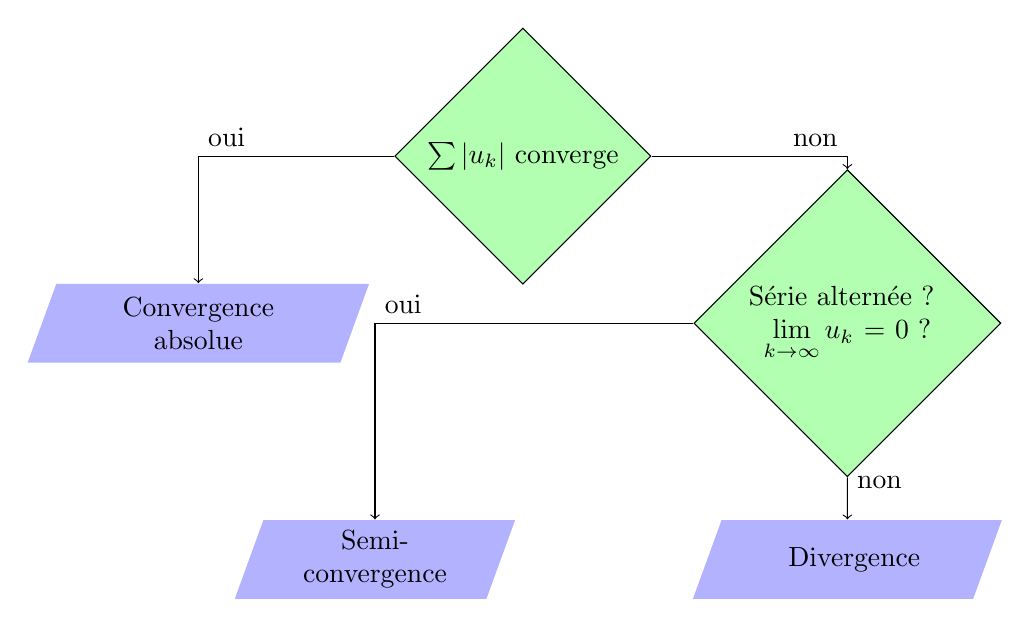
\begin{tikzpicture} [node distance = 3cm]
\node (uniforme) [condition] {$ \sum |u_k| $ converge};
\node (absolue) [input, below left of = uniforme, text width = 3cm, xshift = -2cm] {Convergence absolue};
\node (alternee) [condition, below right of = uniforme, xshift = 2cm, text width = 2.5cm] {Série alternée ? \newline $\displaystyle \lim_{k \to \infty}u_k=0$ ?};

\node (diverge) [input, below of = alternee, text width = 1.5cm] {Divergence};
\node (semi) [input, left of = diverge, text width = 2.5cm, xshift = -3cm] {Semi-convergence};

\draw[->] (uniforme) -| node[anchor=south west]{oui} (absolue);
\draw[->] (uniforme) -| node[anchor=south east]{non} (alternee);
\draw[->] (alternee) -| node[anchor=south west]{oui} (semi);
\draw[->] (alternee) -- node[anchor=south west]{non} (diverge);
\end{tikzpicture}
\end{center}

\begin{itemize}
\item Absolument convergente : Si la série $\displaystyle \sum_{k=1}^{\infty} |u_k| $ converge, alors la série $\displaystyle \sum_{k=1}^{\infty} u_k $ converge également et est dite absolument convergente.
\item Divergente : Si le critère de la racine ou le critère du quotient montre que la série des modules $\displaystyle \sum_{k=1}^{\infty} |u_k| $ diverge, alors la série sans module $\displaystyle \sum_{k=1}^{\infty} u_k $ diverge également.
\item Semi-convergente : Pour qu'une série alternée de la forme $\displaystyle \sum_{k=1}^{\infty} (-1)^k v_k $ soit convergente, il suffit que la suite des $ \{ v_k \} $ tende monotonement vers 0.
\end{itemize}






%% Convergence uniforme
\item Convergence uniforme : Lorsque l'on a une suite ou une série \emph{numérique}, sa convergence définit un nombre. Dans le cas où la suite (ou série) dépend d'une variable $ x $ $\displaystyle \Big( \lim_{k \to \infty} f_k(x) \text{ pour les suites et } \sum_{k=1}^{\infty} f_k(x) \text{ pour les séries} \Big) $, alors elle représente une fonction $ f(x) $ dans le domaine de convergence de la suite (ou série). \\
Une série est uniformément convergente si la suite de ses sommes partielles est uniformément convergente, c-à-d $\displaystyle \sum_{k=1}^{n} f_k \overset{I}{\implies} f $ \quad si et seulement si \quad $\displaystyle (\forall \epsilon > 0) (\exists N) (\forall x \in I, \; \forall n \geq N) : | S_n(x) - f(x) | \leq \epsilon $. \\
Autrement dit, il est possible de rendre la différence entre la série $ S_n $ et la fonction $ f $ arbitrairement petite (puisque $ \epsilon $ peut être infiniment petit) pour tout $ x $ dans l'intervalle $ I $. Plus $ n $ est grand, et plus cette différence sera petite, mais $ n $ doit au minimum prendre la valeur $ N $.





%% Critère de Weierstrass
\item En pratique, la convergence uniforme d'une série de fonction peut être vérifiée par le critère de Weierstass : Si le module du terme général $ f_k(x) $ d'une série de fonctions est majoré par le terme général $ u_k $ d'une série numérique convergente, c-à-d si \qquad $\displaystyle |f_k(x)| \leq u_k, \; \forall x \in I $ \qquad alors la série \qquad $\displaystyle \sum_{k=1}^{\infty} f_k(x) $ \qquad est absolument et uniformément convergente sur $ I $. \\
\emph{Exemple} : $\displaystyle \sum_{k=1}^{\infty} \frac{\cos(k x)}{k^2} $ converge uniformément et absolument (sur $ \mathbb{R} $) puisque $\displaystyle \Big| \frac{\cos(k x)}{k^2} \Big| \leq \frac{1}{k^2} $.





%% Dérivée d'une série de fonctions
\item Condition suffisante pour la dérivation terme à terme d'une série de fonctions :
\[
\left.
    \begin{aligned}
        f_k \in C_1([a, b]) \\
        \exists x_0 \in [a, b], \alpha \in \mathbb{C} : \quad \sum_{k=1}^{\infty} f_k(x_0) = \alpha \\
        \sum_{k=1}^{\infty} f'_k \overset{[a, b]}{\implies} g
    \end{aligned}
\right\}
\qquad \exists f \in C_1([a, b])
\]
Ce qui induit que \qquad (1) $ f(x_0) = \alpha $ \qquad (2) $\displaystyle \sum_{k=1}^{\infty} f_k \overset{[a, b]}{\implies} f $ \qquad (3) $ g = f' $






%% Primitivation d'une série de fonction
\item Primitivation d'une série de fonctions : Si la série $\displaystyle \sum_{k=1}^{\infty} f_k(x) $ de fonctions \big($ f_k(x) \in C_0([a, b]) $\big) converge uniformément vers $ f $ sur l'intervalle $ [a, b] $, alors, $ \forall x_0 \in [a, b] $, 
\[ \sum_{k=1}^{\infty} \int_{x_0}^{x} f_k(t) \; dt \overset{[a, b]}{\implies} \int_{x_0}^{x} f(t) \; dt \]






%% Séries de puissances
\item Une série de puissance est de la forme : $\displaystyle \sum_{k=0}^{\infty} a_k x^k $ \Big( ou de manière plus générale $\displaystyle \sum_{k=0}^{\infty} a_k (x - x_0)^k $ \Big). Les critères du quotient et de la racine permettent l'étude de la convergence d'une série de puissances.





%% Rayon de convergence
\item Le rayon de convergence d'une série est la valeur de $ \rho $ telle que la série converge absolument dans l'intervalle $ ]-\rho + x_0, x_0 + \rho[ $ appelé intervalle de convergence.
\begin{center}
\begin{tikzpicture}
\draw[-] (-5, 0) -- (5, 0);

\node (premier) [rectangle, xshift = -3.5cm] {\bigg]};
\node (second) [rectangle, xshift = 3.5cm] {\bigg[};
\node (centre) [rectangle, yshift = 0.25cm] {$ x_0 $};

\draw[<->] (-3.5, -0.6) -- (0, -0.6);
\node (rho) [rectangle, xshift = -1.75cm, yshift = -0.45cm] {$ \rho $};
\end{tikzpicture}
\end{center}

Les cas particuliers $ \rho = 0 $ et $ \rho = + \infty $ correspondent respectivement à une série de puissances qui converge uniquement en $ x_0 $ et pour tout $ x $ dans $ \mathbb{R} $.





%% Convergence uniforme et absolue d'une série de puissance
\item Convergence uniforme et absolue d'une série de puissance : Toute série de puissance $\displaystyle \sum_{k=0}^{\infty} a_k (x - x_0)^k $ converge uniformément et absolument dans tout intervalle fermé borné strictement compris dans son intervalle de convergence.

Ce résultat révèle toute la force des séries de puissances. Notons $ \tilde{x} $ la limite de l'intervalle de convergence. Non seulement la série de puissances converge sur $ |x − x_0| \leq |\tilde{x} − x_0| $ si elle converge en $ \tilde{x} $ (ce qui justifie la notion d’intervalle de convergence), mais, en plus, la convergence est nécessairement uniforme sur tout intervalle fermé borné de l’intervalle de convergence.

Autrement dit, toutes série de puissances convergeant en une extrémité $ \tilde{x} $ de son intervalle de convergence $ I $ converge également uniformément sur tout intervalle fermé borné $ [\alpha, \beta] \subset I \cup \{ \tilde{x} \} $. Son intervalle de convergence s'étend donc de $\displaystyle I \equiv \; ]-\rho + x_0, x_0 + \rho[ \; \equiv \; ]a, b[ $ \; à \; $\displaystyle I \cup \{ \tilde{x} \} \equiv \; ]a, b] $ (si $ \tilde{x} $ correspond à $ b $).





%% Propriété des séries de puissances
\item Propriété des séries de puissances : Toute série de puissances représente une fonction indéfiniment continûment dérivable sur son intervalle de convergence et peut être dérivée et primitivée terme à terme. \\
Les séries obtenues en dérivant ou en primitivant terme à terme une série de puissances convergent absolument et uniformément sur tout intervalle fermé borné de l’intervalle de convergence de la série initiale. \\
Attention, si on a un intervalle de convergence de la forme $ I \cup \{ \tilde{x} \} \equiv \; ]a, b] $, il faut re-vérifier la convergence au point $ \tilde{x} $.





%% Série de puissances d'une fonction connue
\item Série de puissances d'une fonction connue : 

On connaît déjà la formule de la série géométrique, valable pour tout $ x \in \; ]-1, 1[ $ : 

\begin{tabular}{M{8cm}|M{2cm}|M{4cm}}
$\displaystyle \frac{1}{1-x} = 1 + x + x^2 + ... + x^k + ... = \sum_{k=0}^{\infty} x^k $ & $ \forall x \in \; ]-1, 1[ $ & Série géométrique \cr
$\displaystyle \frac{1}{1+x} = 1 - x + x^2 + ... + (-1)^k x^k + ... $ & $ \forall x \in \; ]-1, 1[ $ & Remplacer $ x $ par $ -x $ \cr
$\displaystyle \ln (1-x) = - x - \frac{x^2}{2} - \frac{x^3}{3} + ... - \frac{x^{k+1}}{k+1} + ... $ & $ \forall x \in \; [-1, 1[ $ & Intégrer $\displaystyle \frac{1}{1 - x} $ \cr
$\displaystyle \ln (1+x) = x - \frac{x^2}{2} + \frac{x^3}{3} + ... + (-1)^k \frac{x^{k+1}}{k+1} + ... $ & $ \forall x \in \; ]-1, 1] $ & Intégrer $\displaystyle \frac{1}{1 + x} $ \cr
$\displaystyle \frac{1}{2} \ln \frac{1+x}{1-x} = x + \frac{x^3}{3} + \frac{x^5}{5} + ... + \frac{x^{2k+1}}{2k+1} + ... $ & $ \forall x \in \; ]-1, 1[ $ & $ = \frac{1}{2} \Big( \ln (1 + x) - \ln (1 - x) \Big) $ \cr
\end{tabular}

\begin{tabular}{M{4.9cm}|M{4.9cm}|M{4.9cm}}
$\displaystyle e^x = \sum_{k=0}^{\infty} \frac{x^k}{k!} $ & $\displaystyle e^{-x} = \sum_{k=0}^{\infty} (-1)^k \frac{x^k}{k!} $ & Toutes ces égalités sont valables pour tout x \cr
$\displaystyle \sinh (x) = \sum_{k=0}^{\infty} \frac{x^{2k+1}}{(2k+1)!} $ & $\displaystyle \sin (x) = \sum_{k=0}^{\infty} (-1)^{k} \frac{x^{2k+1}}{(2k+1)!} $ & Fonctions impaires, exposant impaire \cr
$\displaystyle \cosh (x) = \sum_{k=0}^{\infty} \frac{x^{2k}}{(2k)!} $ & $\displaystyle \cos (x) = \sum_{k=0}^{\infty} (-1)^k \frac{x^{2k}}{(2k)!} $ & Fonctions paires, exposant paire \cr
\end{tabular}

On peut retenir les formules des cosinus et sinus grâce à la parité des fonctions, le cosinus est pair et donc l'exposant du $ x $ est pair et la fonction sinus est impaire et donc l'exposant du terme général est impair. Sinon, ça reste facile à retenir puisque le corps général de la série reste similaire pour toutes ces fonctions trigonométriques. On retient aussi que les fonctions de trigonométrie hyperbolique n'ont pas de facteur $ (-1)^k $. \\ \\ \\ \\






%% Résoudre des équations différentielles
\item \danger Attention !! Pour résoudre des équations différentielles avec des séries, retournez dans le livre, refaites la théorie, les exercices, des problèmes et des exercices d'examens.







\end{itemize}

























\newpage


























\section{Calcul intégral}











\begin{itemize}












%% Critère de Lebesgue
\item Critère de Lebesgue : Toute fonction mesurable $ f $ de module majoré par une fonction intégrable $ F $ est elle même intégrable, soit : 
\[
\left.
    \begin{aligned}
        f \text{ mesurable } \\
        | f | \leq F \in \mathbb{L}_1
    \end{aligned}
\right\}
\implies f \in \mathbb{L}_1
\]
En pratique, toutes les fonctions sont mesurables, et il suffit donc que $ | f | $ soit plus petite ou égale à une autre fonction $ F $ (en fait $ F $ est intégrable elle-même) pour que $ f $ soit intégrable. \\
$ | f | \leq $ Fonction intégrable $ \implies $ $ f $ est intégrable.






%% Conséquence pratique du critère de Lebesgue
\item Conséquence pratique du critère de Lebesgue : Toute fonction $ f $ continue sur un compact $ K \subset \mathbb{R}^n $ est intégrable sur ce compact. \\
Conséquence simple puisque toute fonction continue sur un intervalle est inférieure à une certaine constante $ C $ et que $ C \in \mathbb{L}_1 $.






%% Critère de non-intégrabilité
\item Critère de non-intégrabilité : Si $ f $ et $ g $ sont des fonctions mesurables telles que 
$ g \notin \mathbb{L}_1 $ et $ | f | \geq | g | $, alors $ f \notin \mathbb{L}_1 $. \\
On utilise le critère de Lebesgue à l'envers ici, pour en faire un critère de non-intégrabilité : si $ f $ était intégrable, alors $ g $ serait intégrable également. Puisque $ g $ n'est pas intégrable, alors $ f $ n'est pas intégrable non plus.






%% Second critère de non-intégrabilité
\item Second critère de non-intégrabilité : Si $ f \in C_0(]a, b[) $ et si 
\[ \lim_{\alpha \to a^+, \beta \to b^-} \int_\alpha^\beta f(x) \; d x \quad \text{ n'existe pas (ou est infinie) } \]
alors $ f \notin \mathbb{L}_1(]a, b[) $. \\
En effet, si $ f $ est intégrable au sens de Lebesgue, cette limite doit exister et être finie. Inversement, si la limite n'existe pas ou est est infinie, la fonction $ f $ n'est pas intégrable au sens de Lebesgue.






%% Critères pratiques d'intégrabilité
\item Critères pratiques d'intégrabilité : 
\begin{itemize}
    \item Intégrabilité sur un domaine BORNÉ : Soit une fonction $ f \in C_0(]a, b]) $, où $ a $ et $ b $ sont finis. \\
Si $\displaystyle \exists \alpha < 1 : f(x) = O \bigg[ \frac{1}{(x - \alpha)^\alpha} \bigg] \quad (x \to a^+) $ ce qui est notamment le cas si $ \exists \alpha < 1 $ et $ C \neq 0 $ : \\
$\displaystyle f(x) = o \bigg[ \frac{1}{(x - a)^\alpha} \bigg] $ ou  $\displaystyle f(x) \sim \frac{C}{(x - a)^\alpha} \quad (x \to a^+) $ alors $ f \in \mathbb{L}_1 (]a, b[) $.
    \item Intégrabilité sur un domaine NON BORNÉ : Soit une fonction $ f \in C_0 ([a, + \infty [) $, où $ a $ est fini. \\
Si $\displaystyle \exists \alpha > 1 : f(x) = O \bigg[ \frac{1}{x^\alpha} \bigg] \quad (x \to \infty) $ ce qui est notamment le cas si 
$ \exists \alpha > 1 $ et $ C \neq 0 $ : \\
$\displaystyle f(x) = o \bigg[ \frac{1}{x^\alpha} \bigg] $ ou $\displaystyle f(x) \sim \frac{C}{x^\alpha} \quad (x \to + \infty) $ alors 
$ f \in \mathbb{L}_1 (]a, + \infty[) $
\end{itemize}






%% Critère de Tonelli
\item Critère de Tonelli \footnote{Il y a un troisième sous-critère à Tonelli : $ f $ doit être mesurable. Mais puisque en pratique, toute fonction est mesurable, ignorons le.} : \Big( Le critère de Tonelli assure l'existence de l'intégrale double \Big) \\
$ f(x, y) $ est intégrable sur $ \mathbb{R}^2 $ si : 
\begin{itemize}
    \item La fonction $ | f(x, y) | $ (Attention à bien prendre la norme !) est intégrable par rapport à $ y $ sur $ \mathbb{R} $ pour 
presque tout $ x $ fixé dans $ \mathbb{R} $. \\
    \item La fonction $\displaystyle \int | f(x, y) | \; d y $ est intégrable par rapport à $ x $ sur $ \mathbb{R} $. \\
Autrement dit (pour ce deuxième point), est-ce que $\displaystyle F(x) = \int | f(x, y) | \; d y $ est intégrable par rapport à $ x $ ?
\end{itemize}

Remarque : Le critère de Tonelli fonctionne aussi pour des intervalles qui ne sont pas égaux à $ \mathbb{R} $.






%% Théorème de Fubini
\item Théorème de Fubini : Si $ f(x, y) $ est intégrable, alors : 
\begin{align*}
\iint f(x, y) \; d x \; d y &= \int d x \int f(x, y) \; d y \\
 &= \int d y \int f(x, y) \; d x
\end{align*}






%% Remarque sur Tonelli et Fubini
\item Remarque sur Tonelli et Fubini : Remarquons que le critère de Tonelli et le théorème de Fubini ne forment que des conditions suffisantes d'intégrabilité et de permutation des ordres d'intégration partielle.






%% Calcul d'aire et volume
\item Calcul d'aire et volume : Une aire se calcule avec la formule $\displaystyle A = \iint_\Omega 1 \; d x \; d y = \iint_\Omega d x \; d y $ \\ et le volume avec la formule $\displaystyle V = \iiint_\Omega 1 \; d x \; d y \; d z = \iiint_\Omega \; d x \; d y \; d z $.






%% Réduction des intégrales dans R^n
\item Réduction des intégrales dans $ \mathbb{R}^n $ : 

Ici, une fois qu'on a montré que l'intégrale existe et que l'on peut intégrer dans n'importe quel ordre (Tonelli et Fubini), on fait la réduction directement et on calcule.

Exemple (pg 557) : 

\begin{center}
\includegraphics[width=0.5\textwidth]{images/tetraedre.PNG}
\end{center}

Calculer le volume du tétraèdre : 
\begin{align*}
V = \iiint_\Omega d x \; d y \; d z &= \int_0^a d x \iint_{\Sigma (x)} d y \; d z \\
 &= \int_0^a d x \int_0^{b - \frac{b x}{a}} d y \int_0^{c (1 - \frac{y}{b} - \frac{x}{a})} d z \\
 &= \int_0^a d x \int_0^{b - \frac{b x}{a}} c \bigg( 1 - \frac{y}{b} - \frac{x}{a} \bigg) d y \\
 &= c \int_0^a \bigg[ y - \frac{y^2}{2 b} - \frac{x y}{a} \bigg]_{y=0}^{y=b-\frac{b x}{a}} d x \\
 &= c \int_0^a \bigg( \frac{b x^2}{2 a^2} - \frac{b x}{a} + \frac{b}{2} \bigg) d x \\
 &= \frac{a b c}{6}
\end{align*}






%% Changement de variables
\item Changement de variables : 
\[ f(x) \in \mathbb{L}_1(E) \iff f[x(x')] \; \bigg| \frac{\partial (x)}{\partial (x')} \bigg| \in \mathbb{L}_1 (E') \]
et \[ \int_E d(x) \; d x = \int_{E'} f[x(x')] \; \bigg| \frac{\partial (x)}{\partial (x')} \bigg| \; d x' \]
où $\displaystyle \bigg| \frac{\partial (x)}{\partial (x')} \bigg| $ est le Jacobien du changement de variable.






%% Systèmes de coordonnées
\item Systèmes de coordonnées : \\
\begin{center} \begin{tabular}{M{6cm}M{10cm}}
\begin{center}
\includegraphics[width=5.5cm]{images/sphere.png}
\end{center}
&
\begin{center}
\includegraphics[width=9.5cm]{images/sphere2.png}
\end{center}
\end{tabular} \end{center}

\begin{center}
    \begin{tabular}{|c|cccc|} \hline
        & Cartésien & Polaire & Cylindrique & Sphérique \\ \hline
        $dA$ & $ dx \; dy $       & $ r \; dr \; d \theta $ & / & / \\
        $dV$ & $ dx \; dy \; dz $ & / & $ r \; dr \; d \theta \; dz $ & $ \rho^2 \; \sin \phi \; d \rho \; d \theta \; d \phi $ \\ \hline
    \end{tabular}
\end{center}

\begin{center}
    \begin{tabular}{|c|ccc|} \hline
        & Cartésien & Cylindrique & Sphérique \\
        & $f(x,y,z)$ & $f(r,\theta,z)$ & $f(\rho,\theta,\phi)$ \\ \hline
        $x$ & $x$ & $r \cos\theta$ & $\rho \cos\theta \sin\phi$ \\
        $y$ & $y$ & $r \sin\theta$ & $\rho \sin\theta \cos\phi$ \\
        $z$ & $z$ & $z$ & $\rho \cos\phi$ \\
        $r$ & $\sqrt{x^2+y^2}$ & $r$ & $\rho \sin\phi$ \\
        $\rho$ & $\sqrt{x^2+y^2+z^2}$ & $\sqrt{r^2+z^2}$ & $\rho$ \\
        $\theta$ & $\tan^{-1} \frac{x}{y}$ & $\theta$ & $\theta$ \\
        $\phi$ & $\tan^{-1}\frac{\sqrt{x^2+y^2}}{z}$ & $\tan^{-1}\frac{r}{z}$ & $\phi$ \\ \hline
    \end{tabular}
\end{center}

Comment choisir le système de coordonnées le plus approprié ? De manière générale, si il y a une symétrie sphérique aux limites ou un terme $ x^2 + y^2 + z^2 $ dans la fonction, alors il faut utiliser les coordonnées sphériques. Dans le cas d'une symétrie cylindrique ou s'il y a un terme $ x^2 + y^2 $, on utilise généralement les coordonnées cylindriques. \footnote{Revoir le calcul de la surface d'un tore (forme de donut) pour un système de coordonnées encore différent.}






%% Longueur d'une courbe
\item Longueur d'une courbe : La courbe régulière $ \mathcal{C} $ est de longueur finie lorsque $ \| \textbf{s}'(t) \| \in \mathbb{L}_1(]a, b[) $. \\
La longueur de la courbe est alors définie par : 
\[ L_{\mathcal{C}} = \int_a^b \| \textbf{s}'(t) \| \; dt \]
On peut le voir de la manière suivante : On a une courbe (objet à une dimension) dans un espace à trois dimensions. On fait donc un changement de variable et on se retrouve alors avec la variable $ t $ et le jacobien $ \| \textbf{s}'(t) \| $ (où $ \textbf{s}(t) $ est la représentation paramétrique de la courbe tel que $ \textbf{s}(t) = x(t) \textbf{e}_x + y(t) \textbf{e}_y + z(t) \textbf{e}_z $, \; $ t \in \; ]a, b[ $). \\
Puisqu'on calcule une longueur, l'intégrale que l'on a est : $\displaystyle \int_a^b 1 \; \| \textbf{s}'(t) \| \; d t $.

Remarque : L'intégrale est indépendante de la représentation paramétrique choisie pour la courbe $ \mathcal{C} $.






%% Longueur d'une courbe plane
\item Longueur d'une courbe plane : Dans le cas d'une courbe plane décrite par l'équation cartésienne $ y = f(x) $ où $ x \in \; [a, b] $ et 
$ f \in C_1([a, b]) $, on a successivement 
\[ \textbf{s}(x) = x \textbf{e}_x + f(x) \textbf{e}_y \qquad \textbf{s}'(x) = \textbf{e}_x + f'(x) \textbf{e}_y \]
\[ d s = \sqrt{1 + \big[ f'(x) \big]^2} d x \]
et donc
\[ L = \int_a^b \sqrt{1 + \big[ f'(x) \big]^2} d x \]






%% Intégrale sur une courbe
\item Intégrale sur une courbe : On définit l'intégrale de $ \phi $ sur la courbe régulière $ \mathcal{C} $ par l'expression : 
\[ \int_\mathcal{C} \phi \; d s = \int_a^b \phi [\textbf{s}(t)] \; \| \textbf{s}'(t) \| \; d t \]
à condition sue l'intégrale du second membre existe. \\
Cette formule est plutôt facile à retenir à partir du moment où on comprend sa signification. En fait, on intègre $ \phi $ qui est un \emph{champ scalaire}, autrement dit, une fonction plutôt normale \big(On peut écrire : $ \phi(x, y, z) = \phi[\textbf{s}(t)] $\big).
Et on ne modifie PAS la fonction $ \phi[\textbf{s}(t)] $, en fait, on fait juste un bête changement de variable et on se retrouve avec cette intégrale.
\begin{center} \begin{tabular}{M{7cm}|M{7cm}}
Longueur d'une courbe & Intégrale sur une courbe \cr
\hline
$\displaystyle L_\mathcal{C} = \int_\mathcal{C} d s = \int_a^b \| \textbf{s}'(t) \| \; d t $ & $\displaystyle \int_\mathcal{C} \phi \; d s = \int_\mathcal{C} \phi[\textbf{s}(t)] \; d s = \int_a^b \phi[\textbf{s}(t)] \; \| \textbf{s}'(t) \| \; d t $
\end{tabular} \end{center}






%% Intégrale curviligne
\item Intégrale curviligne : L'expression 
\[ \int_\mathcal{C} \textbf{F}(\textbf{s}) \cdot d \textbf{s} = \int_a^b \textbf{F}[\textbf{s}(t)] \cdot \textbf{s}'(t) \; d t \]
est appelée l'\emph{intégrale curviligne} de $ \textbf{F} $ sur $ \mathcal{C} $ si l'intégrale du second membre existe. \\
C'est une formule qui est très simple à retenir, on ne fait même pas de changement de variable compliqué ici, on fait juste l'opération suivante : 
\[ \int_\mathcal{C} \textbf{F}(\textbf{s}) \cdot d \textbf{s} = \int_a^b \textbf{F}[\textbf{s}(t)] \cdot d \textbf{s}(t) = \int_a^b \textbf{F}[\textbf{s}(t)] \cdot \frac{d \textbf{s}(t)}{d t} \; d t = \int_a^b \textbf{F}[\textbf{s}(t)] \cdot \textbf{s}'(t) \; d t \]

Remarque : L'intégrale curviligne change de signe si on change l'orientation de la courbe : \[ \int_\mathcal{C} \textbf{F} \cdot d \textbf{s} = - \int_{- \mathcal{C}} \textbf{F} \cdot d \textbf{s} \]






%% Calculer une intégrale curviligne
\item Calculer une intégrale curviligne : Formellement, si on décompose $ \textbf{s}(t) $ et $ d \textbf{s} $ en leurs composantes cartésiennes : 
\[ \textbf{s}(t) = x(t) \textbf{e}_x + y(t) \textbf{e}_y + z(t) \textbf{e}_z, \qquad t \in \; [a, b] \]
\[ d \textbf{s} = d x \; \textbf{e}_x + d y \; \textbf{e}_y + d z \; \textbf{e}_z \]
Alors on peut définir les intégrales : 
\[ \int_\mathcal{C} F_x(\textbf{s}) \; d x = \int_a^b F_x(\textbf{s}(t)) \; x'(t) \; d t \]
\[ \int_\mathcal{C} F_y(\textbf{s}) \; d y = \int_a^b F_y(\textbf{s}(t)) \; y'(t) \; d t \]
\[ \int_\mathcal{C} F_z(\textbf{s}) \; d z = \int_a^b F_z(\textbf{s}(t)) \; z'(t) \; d t \]
telles que : 
\[ \int_\mathcal{C} \textbf{F}(\textbf{s}) \cdot d \textbf{s} = \int_\mathcal{C} F_x(\textbf{s}) \; d x + \int_\mathcal{C} F_y(\textbf{s}) \; d y +  \int_\mathcal{C} F_z(\textbf{s}) \; d z \]

Remarque : Avec ces notations, attention à ne pas confondre les expressions du type 
\[ \int_\mathcal{C} F_x \; d x \qquad \text{ et } \qquad \int_a^b F_x \; d x \]






%% La circulation de F
\item La circulation de $ \textbf{F} $ : Si $ \mathcal{C} $ désigne une courbe régulière fermée, l'intégrale curviligne $\displaystyle \int_\mathcal{C} \textbf{F} \cdot d \textbf{s} $ est appelée la circulation de \textbf{F} et est notée : 
\[ \oint_\mathcal{C} \textbf{F} \cdot d \textbf{s} \]






%% Théorème fondamental des intégrales curvilignes
\item Théorème fondamental des intégrales curvilignes : Si $ \mathcal{C} $ désigne un arc régulier de longueur finie d'extrémités $ \textbf{s}_1 $ et $ \textbf{s}_2 $ et inclus dans l'ouvert $ \Omega \subset \mathbb{R}^3 $, si la fonction $ \phi $ est continûment dérivable sur $ \Omega $, alors \[ \int_\mathcal{C} \nabla \phi \cdot d \textbf{s} = \phi(\textbf{s}_2) - \phi(\textbf{s}_1) \]
de sorte que l'intégrale est indépendante du chemin $ \mathcal{C} $ joignant $ \textbf{s}_1 $ et $ \textbf{s}_2 $.






%% Autres intégrales
\item Autres intégrales : Les intégrales précédentes ne sont pas les seules qu'on puisse définir. Ainsi, on écrira encore, en raisonnant éventuellement composante par composante : 
\[ \int_\mathcal{C} \textbf{F}(\textbf{s}) \wedge d \textbf{s} = \int_a^b \textbf{F}(\textbf{s}(t)) \wedge \textbf{s}'(t) \; d t \]
\[ \int_\mathcal{C} \textbf{F}(\textbf{s}) \; d s = \int_a^b \textbf{F}(\textbf{s}(t)) \; \| \textbf{s}'(t) \| \; d t \]
\[ \int_\mathcal{C} \phi(\textbf{s}) \; d \textbf{s} = \int_a^b \phi(\textbf{s}(t)) \; \textbf{s}'(t) \; d t \]
Contrairement aux intégrales précédentes, ces intégrales définissent des grandeurs vectorielles.






%% Formule de Green
\item Formule de Green : Si $ K \subset \mathbb{R}^2 $ est un compact régulier dont la frontière $ \delta K^+ $ constituée d'un ou plusieurs contours réguliers par morceaux est orienté "aire à gauche" et si $ \textbf{F} = F_x \textbf{e}_x + F_y \textbf{e}_y + F_z \textbf{e}_z \in C_1 (K) $, alors 
\[ \iint_K (\nabla \wedge \textbf{F}) \cdot \textbf{e}_z \; d x \; d y = \iint_K \bigg( \frac{\partial F_y}{\partial x} - \frac{\partial F_x}{\partial y} \bigg) \; d x \; d y = \oint_{\partial K^+} \textbf{F} \cdot d \textbf{s} \]
On se retrouve ici avec une formule plus compliquée à retenir. La manière la plus simple de faire est de retenir par coeur (ou de savoir retrouver en faisant un déterminant) ceci : 
\[ \iint_K (\nabla \wedge \textbf{F}) \cdot \textbf{e}_z \; d x \; d y = \iint_K \bigg( \frac{\partial F_y}{\partial x} - \frac{\partial F_x}{\partial y} \bigg) \; d x \; d y \]
Pour arriver à l'étape suivante, on distribue le $ d x $ et le $ d y $, pour obtenir \footnote{On change aussi le domaine d'intégration, on avait la surface $ K $ et maintenant le contour $ \partial K^+ $ (qui entoure $ K $, et est orienté dans le sens anti-horloger). On peut comparer cela au théorème fondamental du calcul intégral : $\displaystyle \int_a^b f'(x) \; d x = f(a) - f(b) $, on fait un calcul sur les limites de l'intervalle ($ a $ et $ b $) et dans un certain sens (on va de $ a $ à $ b $).} : 
\[ \iint_K \bigg( \frac{\partial F_y}{\partial x} - \frac{\partial F_x}{\partial y} \bigg) \; d x \; d y 
= \oint_{\partial K^+} F_x \; d x + F_y \; d y
= \oint_{\partial K^+} \textbf{F} \cdot d \textbf{s} \]






%% Aire d'une surface courbe
\item Aire d'une surface courbe : On définit l'aire d'une surface courbe régulière $ \Sigma $ par la formule : 
\[ S = \iint_\Sigma d \sigma = \iint_\Omega \bigg\| \frac{d \textbf{s}}{d u} \wedge \frac{d \textbf{s}}{d v} \bigg\| \; d u \; d v \]
si cette intégrale existe, c-à-d si : 
\[  \bigg\| \frac{d \textbf{s}}{d u} \wedge \frac{d \textbf{s}}{d v} \bigg\| \in \mathbb{L}_1(\Omega) \]






%% Surface de révolution
\item Surface de révolution : Si une surface est engendrée par la rotation d'une courbe plane $ y = f(x) \geq 0 $ autour de l'axe OX, on peut introduire le paramétrage, 
\[ \textbf{s}(x, \theta) = x \textbf{e}_x + f(x) \cos(\theta) \textbf{e}_y + f(x) \sin(\theta) \textbf{e}_z, \qquad x \in \; ]a, b[, \; \theta \in \; ]0, 2 \pi[ \]
de sorte que 
\[ d \sigma = \bigg\| \frac{d \textbf{s}}{d x} \wedge \frac{d \textbf{s}}{d \theta} \bigg\| \; d x \; d \theta = f(x) \sqrt{ 1 + [f'(x)]^2 } \; d x \; d \theta \]


%   Explication => lignes sur les cotés

\begin{siderules}

puisque, 
\[ \frac{d \textbf{s}}{d x} = \textbf{e}_x + f'(x) \cos \theta \;  \textbf{e}_y + f'(x) \sin \theta \; \textbf{e}_z
\quad \text{ et } \quad \frac{d \textbf{s}}{d \theta} = - f(x) \sin \theta \; \textbf{e}_y + f(x) \cos \theta \; \textbf{e}_z \]

\begin{align*}
\frac{d \textbf{s}}{d x} \wedge \frac{d \textbf{s}}{d \theta} = 
\begin{vmatrix}
1 & f'(x) \cos \theta & f'(x) \sin \theta \cr
0 & - f(x) \sin \theta & f(x) \cos \theta \cr
\textbf{e}_x & \textbf{e}_y & \textbf{e}_z \cr
\end{vmatrix}
&= \bigg( f(x) f'(x) \cos^2 \theta + f(x) f'(x) \sin^2 \theta \bigg) \textbf{e}_x \cr
&+ \bigg( - f(x) \cos \theta \bigg) \textbf{e}_y
+ \bigg( f(x) \sin \theta \bigg) \textbf{e}_z \cr
\end{align*}
Et puisque $ \cos^2\theta + \sin^2\theta = 1 $, on a la simplification, 
\[ \frac{d \textbf{s}}{d x} \wedge \frac{d \textbf{s}}{d \theta} = f(x) f'(x) \; \textbf{e}_x - f(x) \cos \theta \; \textbf{e}_y + f(x) \sin \theta \; \textbf{e}_z \]
On arrive donc bien à la formule : 
\[ d \sigma = \bigg\| \frac{d \textbf{s}}{d x} \wedge \frac{d \textbf{s}}{d \theta} \bigg\| \; d x \; d \theta = f(x) \sqrt{ 1 + [f'(x)]^2 } \; d x \; d \theta \]

\end{siderules}


Nous avons donc la formule pour la surface : 
\begin{align*}
S &= \iint_\Sigma d \sigma = \iint_\Omega \bigg\| \frac{d \textbf{s}}{d u} \wedge \frac{d \textbf{s}}{d v} \bigg\| \; d u \; d v \cr
&= \int_0^{2\pi} \int_a^b f(x) \sqrt{1 + \big[f'(x)\big]^2} \; d x \; d \theta \cr
&= 2 \pi \int_a^b f(x) \sqrt{1 + \big[ f'(x) \big]^2} \; d x
\end{align*}






%% Intégrale sur une surface
\item Intégrale sur une surface : Si $ \phi (\textbf{s}) $ désigne un champ scalaire défini sur la surface régulière $ \Sigma $, on définit l'intégrale de $ \phi $ sur la surface par la formule : 
\[ \iint_\Sigma \phi \; d \sigma = \iint_\Omega \phi[\textbf{s}(u, v)] \; \bigg\| \frac{\partial \textbf{s}}{\partial u} \wedge \frac{\partial \textbf{s}}{\partial v} \bigg\| \; d u \; d v \]
à condition que l'intégrale du second membre existe.






%% Théorème de Gauss dans R^2
\item Théorème de Gauss dans $ \mathbb{R}^2 $ : Si $ K \in \mathbb{R}^2 $ est un compact régulier dont la frontière $ \partial K^+ $ constituée d'un ou plusieurs contours réguliers par morceaux est orienté "aire à gauche" et si $ \textbf{F} \in C_1(K) $, alors 
\[ \iint_K \nabla \cdot \textbf{F} \; d x \; d y = \oint_{\partial K^+} \textbf{F} \cdot \textbf{n} \; d s \]
où $ \textbf{n} $ désigne la normale unitaire extérieure à $ K $. \\
Le théorème de Gauss (dans $ \mathbb{R}^2 $, mais aussi dans $ \mathbb{R}^3 $ ou $ \mathbb{R}^n $ une fois généralisé) est un corollaire \footnote{Un corollaire est une proposition qui se déduit immédiatement d'une proposition déjà démontrée. Fait résultant inévitablement d'un autre fait ; conséquence.} important de la \emph{formule de Green}. \\
En fait, on sait que $ \nabla \cdot \textbf{F} = \frac{d F_x}{d x} + \frac{d F_y}{d y} $ ce qui correspond (si on considère que $ \textbf{F} $ est une force) à la \emph{vitesse} d'une particule traversant la surface $ K $. \footnote{Étant donné qu'une force est proportionnelle à une accélération avec $ \vec{\textbf{F}} = m \vec{\textbf{a}} $, alors il est légitime de dire que $ \nabla \cdot \vec{\textbf{F}} $ est une vitesse.} \\
Quant à $ \textbf{F} \cdot \textbf{n} $, c'est la norme de la composante de $ \textbf{F} $ dans la direction normale $ \textbf{n} $. Et on intègre sur le contour de la surface parce que $ \textbf{F} \cdot \textbf{n} $ est la \emph{vitesse} d'une particule (ou d'un corps) passant au travers de TOUTES les surfaces délimitées par $ \partial K^+ $. \footnote{$ \partial K^+ $ est orienté à cause du "+", parce que c'est un contour en deux dimensions et qu'il faut bien que il y ait un sens positif, un début et une fin pour calculer l'intégrale (on paramétrise généralement la courbe $ \partial K $ avec un angle $ \theta $ orienté qui donne une orientation à $ \partial K^+ $).}






%% Théorème de Gauss dans R^3
\item Théorème de Gauss dans $ \mathbb{R}^3 $ : Si $ K \subset \mathbb{R}^3 $ est un compact régulier dont la frontière $ \partial K^+ $ est constituée d'une ou plusieurs surfaces fermées régulières par morceaux et si $ \textbf{F} \in C_1(K) $, alors 
\[ \iiint_K \nabla \cdot \textbf{F} \; d x \; d y \; d z = \iint_{\partial K} \textbf{F} \cdot d \boldsymbol{\sigma} = \iint_{\partial K} \textbf{F} \cdot \textbf{n} \; d \sigma \]
où $ \textbf{n} $ désigne la normale extérieure à $ K $. \\
La formule de Gauss dans $ \mathbb{R}^3 $ est assez similaire à celle de Gauss dans $ \mathbb{R}^2 $, on retient juste que : 
$\displaystyle \textbf{n} \; d \sigma = d \boldsymbol{\sigma} $, 
\[ \textbf{n} = \frac{\displaystyle \frac{\partial \textbf{s}}{\partial u} \wedge \frac{\partial \textbf{s}}{\partial v} }{\displaystyle \bigg\| \frac{\partial \textbf{s}}{\partial u} \wedge \frac{\partial \textbf{s}}{\partial v} \bigg\| }, \qquad \qquad 
d \boldsymbol{\sigma} = \textbf{n} \; d \sigma = \frac{\displaystyle \frac{\partial \textbf{s}}{\partial u} \wedge \frac{\partial \textbf{s}}{\partial v} }{\displaystyle \bigg\| \frac{\partial \textbf{s}}{\partial u} \wedge \frac{\partial \textbf{s}}{\partial v} \bigg\| } \; \bigg\| \frac{\partial \textbf{s}}{\partial u} \wedge \frac{\partial \textbf{s}}{\partial v} \bigg\| \; d r \; d \theta \]






%% Théorème de Stokes
\item Théorème de Stokes : Si $ \textbf{F} $ est un champ vectoriel continûment dérivable sur un ouvert contenant la surface $ \Sigma $ régulière par morceaux, alors 
\[ \iint_\Sigma (\nabla \wedge \textbf{F}) \cdot \textbf{n} \; d \sigma = \oint_{\partial \Sigma} \textbf{F} \cdot d \textbf{s} \]
où $ \partial \Sigma $ désigne le contour de la surface $ \Sigma $ orienté dans le sens compatible avec la règle de la main droite appliquée à la normale $ \textbf{n} $.
En fait, le théorème de Stokes est la généralisation de la formule de Green aux surfaces non planes (donc rien de difficile à retenir).








\newpage








%% Surface d'un tore
\item Surface d'un tore : 

\begin{center}
  \makebox[\textwidth]{
    \includegraphics[width=0.55\paperwidth]{images/tore.PNG}
    \includegraphics[width=0.3\paperwidth]{images/tore2.jpg}
}
\end{center}

Calculons la surface d'un tore obtenu en faisant tourner un cercle de rayon $ a $ autour d'un axe situé à une distance $ R $ de son centre ($ R > a $). \\
En utilisant les vecteurs unitaires des coordonnées cylindriques, la surface est décrite par : 
\[ \textbf{s}(\theta, \phi) = \big( R + a \cos \phi \big) \; \textbf{e}_r(\theta) + a \sin \theta \; \textbf{e}_z, \qquad \theta \in \; ]0, 2 \pi[, \; \; \phi \in \; ]0, 2 \pi[ \]
de sorte que 

\begin{align*}
d \sigma &= \Big\| \big( R + a \cos \phi \big) \; \textbf{e}_\theta \wedge \big( - a \sin \phi \; \textbf{e}_r + a \cos \phi \; \textbf{e}_z \big) \Big\| \; d \theta \; d \phi \cr
&= \big( R + a \cos \phi \big) a \; d \theta \; d \phi
\end{align*}
Il vient dés lors 
\[ S = \int_0^{2 \pi} d \theta \int_0^{2 \pi} \big( R + a \cos \phi \big) a \; d \phi = 4 \pi^2 R a \]











\end{itemize}







































































\end{document}
